\section{DRAGR}
\label{sDRAGR}

\hypertarget{sDRAGRhy}{The}
DRAGR\index{DRAGR|textbf} module is used to prepare libraries for the
reactor-physics code DRAGON\cite{PIP2009,dragon}.\index{DRAGON}
DRAGON is a 1D/2D/3D lattice code developed at \'Ecole Polytrchnique de
Montr\'eal since 1990 and is currently available under an open source
license. DRAGON5, released in 2014, is a 64-bit clean version of the
code, written in Fortran 2003 around an ANSI C kernel\cite{dragon5}.

DRAGON is able to access any standard MATXS-type library (both from NJOY-89
and subsequent versions), as produced by NJOY, using the cross-section
reconstruction algorithm of the code TRANSX-2\cite{TRANSX2}. DRAGON also
has capabilities to use cross-section libraries in the WIMS-AECL, WIMS-D,
APOLLO and Draglib formats. The DRAGR module is dedicated to the production
of cross-section libraries in the Draglib format.

This chapter of the report describes DRAGR in NJOY 2012.0.
It differs from the version previously reported
because of the change to Fortran-90 style and storage allocation.

\subsection{An overview of DRAGR}\label{sect:dragr}

The DRAGR module was written as a clean and direct utility to format a Draglib
library, using PENDF and GENDF data. Care was taken to avoid unnecessary
processing of nuclear data and to keep the richness of ENDF/B information.
Other advantages are related to the use of the Draglib format, thanks to the
careful design of its direct access procedure. The cross-section processing in
DRAGR is similar to the  approach used in module \uppercase{matxsr}. The basic
principle is to avoid unnecessary approximations or simplifications. A Draglib
features the following characteristics:
\begin{itemize}
\item The library file can be converted back and forth between a sequential
ASCII format and a binary direct access format. DRAGR contains all management
capabilities built-in.
\item The steady-state fission spectrum, $\chi(g)$, is assumed to be dilution
independent. It is calculated using
\begin{equation}
\chi(g)={\sum\limits_h \sigma_{\rm f}(g \leftarrow h) \phi_0(h) \over
\sum\limits_g\sum\limits_h\sigma_{\rm f}(g \leftarrow h) \phi_0(h)}
\label{eq:eq1_605}
\end{equation}

where $\sigma_{\rm f}(g \leftarrow h)$ and $\phi_0(h)$, the library weight
function for the first Legendre order,  are recovered from {\tt MF=6} and
{\tt MT=18} records of the GENDF file.

\vskip 0.08cm

The steady-state $\nu\sigma_{\rm f}$ values are calculated using
\begin{equation}
\nu\sigma_{\rm f}(g)=\sum_h \sigma_{\rm f}(h \leftarrow g) .
\label{eq:eq1_606}
\end{equation}

\vskip 0.08cm

The delayed fission spectra, $\chi^{\rm del}_\ell(g)$, are assumed to be
dilution independent. They are calculated using
\begin{equation}
\chi^{\rm del}_\ell(g)={ \nu^{\rm del}_\ell(g)\over
\sum\limits_h\nu^{\rm del}_\ell(h) }
\label{eq:eq1_607}
\end{equation}

where $\nu^{\rm del}_\ell(g)$ is recovered from {\tt MF=5} and {\tt MT=455}
record of the GENDF file.

\vskip 0.08cm

The delayed $\nu\sigma_{\rm f}$ values are calculated using
\begin{equation}
\nu^{\rm del}\sigma_{{\rm f},\ell}(g)=\pi(g)\left(
\sum_h\nu^{\rm del}_\ell(h)\right)\sigma_{\rm f}(g)
\label{eq:eq1_608}
\end{equation}

where $\pi(g)$ is recovered from {\tt MF=3} and {\tt MT=455} record of the
GENDF file and $\sigma_{\rm f}(g)$ is recovered from {\tt MF=3} and {\tt MT=18}
record of the GENDF file.

\item The scattering matrix for the first Legendre order,
$\sigma_{\rm scat0}(h \leftarrow g)$, describes the energy transfer that follows
an isotropic collision in the LAB. The collision can be an elastic or inelastic
diffusion, a (n,2n), or a (n,3n) reaction. It is calculated from GENDF file
information, using
\begin{equation}
\sigma_{\rm scat0}(h \leftarrow g)=\sigma_{\rm diffusion}(h \leftarrow g)+
\sigma_{\rm n,2n}(h \leftarrow g)+\sigma_{\rm n,3n}(h \leftarrow g)
\label{eq:eq1_609}
\end{equation}

This matrix is stored using the sparse storage scheme of the MATXS format,
with the help of two $h$-indexed vectors:
\vskip -0.8cm
\begin{eqnarray*}
i_{\rm scat0}(h) \negthinspace\negthinspace &=& \negthinspace\negthinspace
\hbox{most thermal group index that can produce a secondary neutron} \\
&~&  \negthinspace\negthinspace\hbox{in group $h$;} 
\\
n_{\rm scat0}(h) \negthinspace\negthinspace &=& \negthinspace\negthinspace
\hbox{number of primary groups that can produce a secondary neutron} \\
&~& \negthinspace\negthinspace \hbox{in group $h$.} 
\end{eqnarray*}

The scattering matrices for subsequent Legendre orders are stored in a similar
manner. No transport-corrected data is written in the Draglib file; the task
of transport correction is handled in the lattice code.

\item The thermal cross sections and scattering matrices depend upon the
binding between the atoms of the material. For the heavier materials, it
is often a good approximation to treat the atoms as a gas of free particles
at an appropriate temperature. Thermal cross sections with coherent or
incoherent effects are included in the GENDF file in addition to the ordinary
static cross sections. To prepare a corrected set of cross sections, DRAGR
modifies the total cross section by subtraction of the static elastic cross
section and by addition of the appropriate incoherent and coherent thermal
cross sections over the thermal energy range. For the scattering matrix,
DRAGR uses the static matrix above the thermal cut-off energy and the
requested incoherent or coherent matrices below.

\item The (n,2n) and (n,3n) cross sections are edited from the GENDF file using

\begin{equation}
\sigma_{\rm n,2n}(g)={1 \over 2}\sum_k \sigma_{\rm n,2n}(k \leftarrow g) \
\ \ {\rm and} \ \ \  \sigma_{\rm n,3n}(g)={1 \over 3}\sum_k
\sigma_{\rm n,3n}(k \leftarrow g)
\end{equation}

\item DRAGR offers the possibility of including PENDF-type information in the
Draglib file, to perform a more accurate self-shielding calculation in the
resolved energy domain. PENDF information is transformed into piecewise uniform
cross sections defined over micro-energy groups, named {\sl Autolib data},
which form a superset of the original group structure.

\item File 8 of ENDF evaluation contains half-lives, decay modes, decay
energies, and radiation spectra for most isotopes. Information concerning
the decay of the reaction products is also given in this file. In addition,
fission product yield data ({\tt MT=454} and {\tt 459}) for fissionable
materials and spontaneous radioactive decay data ({\tt MT=457}) for the
nucleus are included.

\vskip 0.08cm

File 8 is processed by module DRAGR. A large number of fission products are
included in
the evaluated file for each element capable of undergoing fission. For example,
in the fission product
yield data file included in ENDF/B-VI rel. 8, one can notice that there is
information of 1232 fission
products for 0.0253 eV fission of $^{233}$U, 1247 fission products for 0.0253
eV fission of $^{235}$U etc. But the
evaluations are not available for all the nuclides, as most of them have very
short half-lives, which in the
reactor context can be considered insignificant. They are subsequently lumped
by a procedure that is
built into DRAGR, as depicted in Fig.~\ref{fig:lumped}. If there are nuclides
with long half-lives, but which are not available as evaluated files, a warning
is provided before lumping the corresponding element. The DRAGR user has
complete control over the lumping process. DRAGR currently has no capability
to produce pseudo-fission product, i.e., custom library isotopes made from
the combination of many minor ENDF fission products.

\vskip 0.08cm

%
\begin{figure}[h!]
\centering
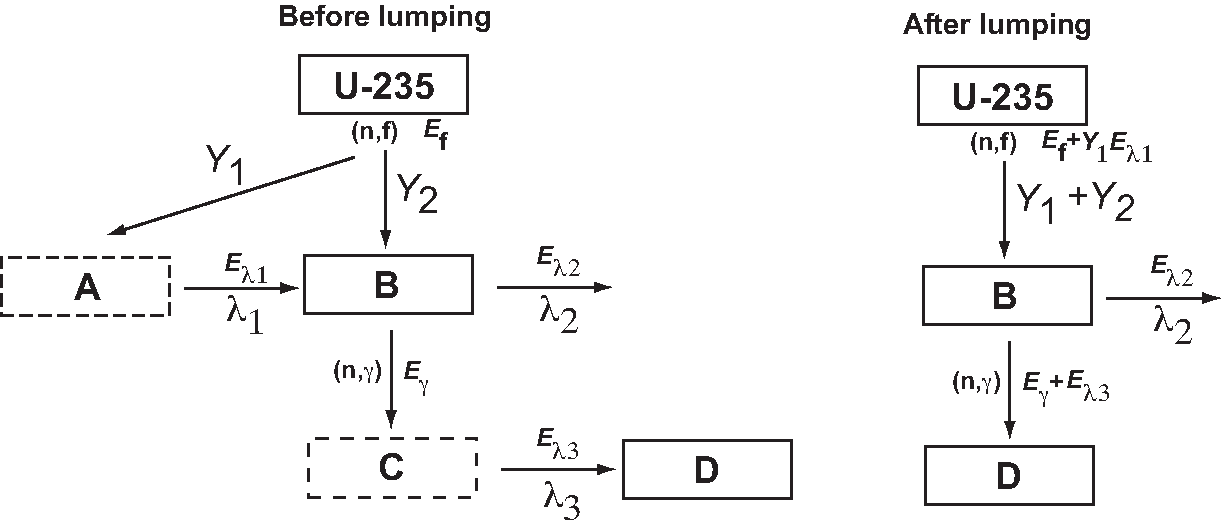
\includegraphics[scale=0.5]{figs/lumped.pdf}
\parbox{11cm}{\caption{Lumping short-lived fission products in $^{235}$U.}
\label{fig:lumped}}   
\end{figure}
%

Information on energies for various reaction types like (n, $\gamma$),
\mbox{(n, f)}, \mbox{(n, 2n)}, \mbox{(n, 3n)}, \mbox{(n, 4n)},
\mbox{(n, $\alpha$)}, (n, p), (n, 2$\alpha$), (n, np), (n, d) and (n, t)
are recovered from earlier DRAGR single-isotope calculations and used for
inclusion in relevant depletion data in Draglib format. The fission energy
of (n, f) is obtained from {\tt MF=1} and {\tt MT=458} and the energy from
delayed betas and gammas is subtracted from it. Information regarding
energies for other reactions is derived by DRAGR from {\tt MF=3}. The
corresponding {\tt MT} numbers for the above-mentioned reactions (other
than (n, f)) are 102, 16, 17, 37, 107, 103, 108, 28, 104, 105, respectively.
The complete information required to do the depletion calculations is
provided in specific records of the Draglib file.

\end{itemize}

\subsection{User Input}
\label{ssDRAGR_inp}

The following user input specifications were copied from the comment
cards at the beginning of the DRAGR source.  It is always a good idea
to check the comment cards in the current version to see if there
have been any changes.
\index{DRAGR!DRAGR input}
\index{input!DRAGR}

\small
\begin{ccode}

   !-----------------------------------------------------------------
   !
   !     Produce a draglib interface file from Njoy intermediate
   !   cross-section library.
   !
   !     The draglib format provide an efficient way to store multi-
   !   group isotopic nuclear data to be used in a lattice code.
   !   For example the draglib can then be used by the Dragon code.
   !
   !     Working from thermr and groupr output tape,this module
   !   produce the standard interface file on the xsm file. The xsm
   !   data base is used to organize the data in a hierarchical
   !   format. Therefore, it will be easy to convert back and forth
   !   between the binary direct access format (efficient during a
   !   calculation) and the ascii or binary format (useful for
   !   backup and exchange purposes).
   !
   ! Authors: Hasan Saygin (original version -- 1992)
   !          Alain Hebert (reprogrammed in 2003)
   !          Alain Hebert (adapted to Njoy2012 in 2014)
   !          Richard Chambon (Multiprocessing in Python -- 2019)
   !
   ! Copyright:
   !  Copyright (C) 2003 Ecole Polytechnique de Montreal
   !  This library is free software; you can redistribute it and/or
   !  modify it under the terms of the GNU Lesser General Public
   !  License as published by the Free Software Foundation; either
   !  version 2.1 of the License, or (at your option) any later
   !  version.
   !
   !---input specifications (free format)----
   !
   ! card 1 file units
   !   nendf     input endf unit
   !   npendf    input pendf unit
   !   ngendf    input gendf unit
   !   nfp       input endf unit for fission yield data
   !   ndcy      input endf unit for radioactive decay data
   !   nimpo     input draglib unit
   !   nexpo     output draglib unit
   !   pfflag    fission product flag: off/on = 0/1. pfflag=1 to
   !             avoid storing scattering matrices. (default=0)
   ! card 2 hollerith identification for the library
   ! (nimpo=0 only)
   !   labell    72 character identification for the library
   ! card 3 material data (one card per material)
   !   matno     integer material identifier
   !             (endf/b mat number)
   !   hmat      hollerith material identifier (up to 8 characters
   !             each). By default, an ascii identifier is
   !             constructed.
   !   nbesp     zero (no energy-dependent fission spectra) or
   !             number of energy-dependent fission spectra)
   ! card 4 material readme comment (up to 72 characters)
   ! card 5 energy mesh for energy-dependent fission spectra
   ! present if and only if nbesp.ne.0
   !   e1, e2, e3, etc. nbesp+1 increasing values of energies (eV)
   ! card 6 energy limits for dilution-dependent xs data. This data
   !        is important to avoid self-shielding in very low and
   !        very high energy group xs and to reduce the size of the
   !        draglib. (one card per material)
   !   eres0     lower limit of resolved resonance xs data (ev)
   !   eres1     upper limit of unresolved resonance xs data (ev)
   ! card 7 autolib energy limits. This data is used with advanced
   !        self-shielding models such as the Sanchez-Coste and
   !        Ribon extended models. It is highly recommended to use
   !        the same data for all resonant isotopes. (one card per
   !        material)
   ! present if and only if npendf.ne.0
   !   eaut0     lower limit of autolib resonance xs data (ev)
   !   eaut1     upper limit of autolib resonance xs data (ev)
   !   deli      elementary lethargy width (ev)
   !
   !            repeat cards 3 to 7 for all materials desired
   !            matno=0/ terminates dragr run.
   !
   ! card 8 burnup chain data (one or two cards per isotope)
   ! present if and only if nfp.ne.0 and ndcy.ne.0
   !  hich      hollerith isotope identifier (same as hmat below)
   !            hich must be constructed in a way compatible with
   !            subroutine dranam (ex: Am242m). If an isotope is
   !            missing in this burnup chain, an error message of
   !            the type 'isotope xxx should not be lumped' may be
   !            issued by subroutine dralum.
   !  hrch(1)   hollerith neutron-induced reaction identifier for
   !            first daughter
   !  en(1)     Q value in MeV for first daughter
   !  br(1)     branching ratio for an isomeric daughter (=0.0 if
   !            there is no isomeric daughter)
   !  hrch(2)   hollerith neutron-induced reaction identifier for
   !            second daughter
   !  en(2)     Q value in MeV for second daughter
   !  ...
   !
   !            repeat card 7 for all isotopes present in the
   !            burnup chain. hich='end'/ terminates the chain.
   !
   ! card 9 concatenate information
   !   hmat      hollerith material identifier (up to 8 characters
   !             each). By default, an ascii identifier is
   !             constructed. It corresponds to the unique isotope 
   !             draglib previously computed that need to be concatenate.
   !   inew      flag to specify if the isotope is the first one. or 
   !             if a concatenated drag lib exist
   !-----------------------------------------------------------------

\end{ccode}
\normalsize

The first card specifies the input and output unit numbers, as
is normal for NJOY modules.  \cword{ngendf} comes from a previous
\hyperlink{sGROUPRhy}{GROUPR} run, and it can be in
either binary or ASCII mode.
Before the multiprocessor version, \cword{nimpo} and \cword{nexpo} 
were always in ASCII mode. Now, they can also be in binary mode.

Card 2 is a comment required if and only if the Draglib is created.

Card 3 is required.  It gives the ENDF MAT number for
the materials to be processed.  If this MAT doesn't appear on
the GENDF tape, a fatal error message will be issued. \cword{hmat}
is the isotope character name on the Draglib. \cword{nbesp} is
generally set to zero, except for libraries dedicated to fast
reactor applications where it is set to 5.

Card 4 is a comment for the isotope.

Card 5 is required only if \cword{nbesp} is not equal to zero.

Card 6 is used to limit the self-shielding domain on the Draglib between
energies \cword{eres0} and \cword{eres1} in eV.

Card 7 is required if and only if \cword{npendf} is not equal to zero.
This information is used to define how the pendf data is transformed
into Autolib data in the Draglib.

Repeat cards 3 to 7 for all materials desired and set \cword{matno=0/}
to terminates the DRAGR run.

Another data group of input data is defined by card 8. This card
permit the definition of depletion chains in the Draglib by gathering
information from endf units \cword{nfp} and \cword{ndcy} containing
fission yield and radioactive decay data, respectively. Repeat card 7
for all isotopes present in the burnup chain. Set \cword{hich='end'/}
to terminates the chain.

The final group of input data is defined by card 9. This card
allows the concatenation of unique isotope draglib into a single file. 
This card is only read if nendf, npendf, ngendf, nfp and ndcy are 0 in 
card 1. Then it replaces card 3.

\cleardoublepage
